In this chapter, we will discuss the obtained results in the process of firmware acquisition and firmware extraction, previous steps before the actual firmware re-hosting.

\section{Firmware acquisition}

For the firmware acquisition, we used a fork of the Firmadyne's \cite{firmadyne} original scraper \cite{github:scraper}. This modified scraper version has fixed some compatibility issues the original scraper has with Python 3 and also updates the spiders to match more updated version of vendor websites. Without modifying any of the spiders provided by the scraper, we selected five vendors and executed the scraper to automatically find and download firmware from these vendors websites. In total, 5265 firmware images were downloaded throughout this process. Table \ref{tab:scraper} show the amount of firmware images and its combined file size for each vendor.

\begin{table}[h]
\centering
\caption{Downloaded firmware images per vendor}
\begin{tabular}{|c|c|c|}
\hline
\textbf{Vendor} & \textbf{Firmware Images} & \textbf{Combined File Size} \\ \hline
Netgear         & 3122                     & 93 GB                       \\ \hline
TP-Link         & 1320                     & 10 GB                       \\ \hline
D-Link          & 430                      & 6.7 GB                      \\ \hline
Ubiquiti        & 226                      & 20 GB                       \\ \hline
Tenda           & 167                      & 1 GB                        \\ \hline
\end{tabular}
\label{tab:scraper}
\end{table}

As the goal of this work is towards the process of re-hosting, this amount of firmware images is already enough for initial experiments with automated re-hosting. In further work, more vendors pages can be extracted, and we can update scraper's spiders if we judge there is need for a larger volume of firmware images.

\section{Firmware extraction}

Firmware extraction was heavily based on the usage of the {\tt binwalk} tool, whose usage was wrapped inside a script provided by Firmadyne \cite{firmadyne}. This script, when executed with a firmware image as a parameter, recursively tries to extract files using {\tt binwalk} for this purpose. It defines a breadth and depth limit to this recursion strategy. During the extraction process, the script then tries to identify if any of the extracted directories has a Linux root directory structure (i.e. has {\tt /bin}, {\tt /etc}, {\tt /usr} directories and so on). If that is the case, then this filesystem structure is compressed and stored in a separate location (also defined as a parameter to the script). 51.17\% of the total amount of firmwares (2694 images) were successfully extracted by Firmadyne's \cite{firmadyne} extraction script. Of these extracted images, 48.52\% (1307 images) had the filesystem extracted and of these, 83.55\% (1092 images) had the architecture identified. Architecture identification is done by reading files in filesystem directories that should contain binary files (e.g. {\tt /bin} or {\tt /sbin}) and reading the header of these files.

Kernel detection is done by reading each entry identified by {\tt binwalk} in the extraction process and detecting known kernel types. These are also extracted and stored in a separate location. When using the script, the user has the option to disable kernel extraction, as this greatly improves execution speed since {\tt binwalk} spends a lot of effort in the extraction process. If kernel extraction is not disabled by user, then the script also tries to identify kernel version and store this information in Firmadyne's \cite{firmadyne} database if found.

As not all kernels are identified by the described process above, we also developed an additional script that uses regular expressions to search the extracted filesystem of each firmware image with a non identified kernel during extraction and for directories that could reveal kernel version (e.g. {\tt /lib/modules/2.6.31} is an indicative that this image contains a 2.6.31 Linux kernel). This search is extremely fast compared to the filesystem extraction process and increased the number of kernel versions detected. Initially, with the Firmadyne's \cite{firmadyne} original extraction script, 983 kernels were identified amongst the 2694 (36.49\%) of the total amount of firmware images. After running the described heuristics to determine kernel version from filesystem, the number of identified kernels increased to 1169 (18.92\% greater).

\begin{figure}[h]
    \centering
    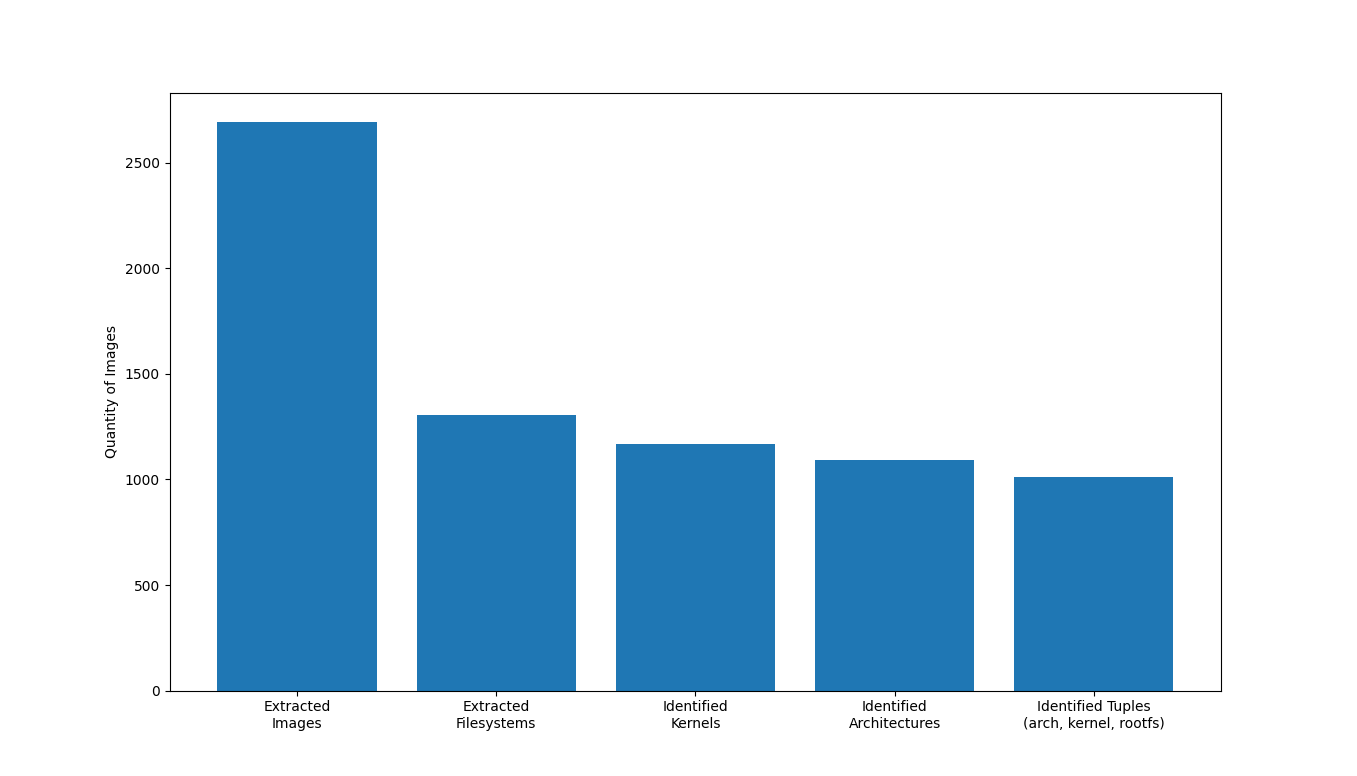
\includegraphics[width=0.90\textwidth]{figs/Funnel.png}
    \caption{Success funnel for firmware image extraction.}
    \label{fig:stats-funnel}
\end{figure}

It was also identified two issues in the extraction process. Some kernel image media types (formerly known as MIME types) were incorrectly identified as a type that was on the extraction script blacklist. This could be easily corrected excluding the identified type from the blacklist. The second issue is related to the recursive extraction process. The limits in breadth and depth exploration allow the {\tt binwalk} tool to have usable performance, but in some cases these limits were in fact responsible for the firmware extraction to be unsuccessful. Therefore, we believe using an heuristic to select files with the most potential to hold firmware kernel or filesystem to be extracted next. This way we can still have breadth and depth limits to maintain the extraction process feasible but it would also focus the extraction in files that are more prominent. This approach of using an heuristics although idealized was not yet implemented in our work.

Another enhancement we developed to the extraction process was the ability to extract addition kernel information. During kernel extraction, the kernel binary file is scanned for ASCII strings and from the result of this search we then extract kernel banner (a string containing kernel version, compiler version used during kernel compilation, compilation date and email of the developer who compiled the kernel) or identify for instance if the system being extracted refers to an OpenWrt Linux. These additional pieces of information are also stored in Firmadyne's \cite{firmadyne} database, that had its schema altered to contain a new column to store the extra information for a given firmware image.

% Falar das estatísticas; Colocar tabela com as estatísticas

\subsection{Statistics}

Regarding firmware extraction and feature identification, we collected some statistics that may help the following steps of this work in kernel compilation and firmware re-hosting. Table \ref{tab:arch-stats} shows the amount of firmwares detected for each architecture identified. Tables \ref{tab:kernel-stats} and \ref{tab:kernel-family-stats} shows the five most common kernel versions and kernel families respectively.

\begin{table}[h]
\centering
\caption{Number of images identified for each found architecture}
\begin{tabular}{|c|c|}
\hline
\textbf{Architecture} & \textbf{Quantity of Images} \\ \hline
{\tt mipseb}                & 485                         \\ \hline
{\tt armel}                 & 336                         \\ \hline
{\tt mipsel}                & 249                         \\ \hline
{\tt mips64eb}              & 11                          \\ \hline
{\tt ppceb}                 & 10                          \\ \hline
{\tt intel64el}             & 1                           \\ \hline
\end{tabular}
\label{tab:arch-stats}
\end{table}

\begin{table}[h]
\centering
\caption{Five most common kernel versions found in extracted firmwares}
\begin{tabular}{|c|c|}
\hline
\textbf{Kernel Version} & \textbf{Quantity of Images} \\ \hline
2.6.31                  & 167               \\ \hline
2.6.36                  & 122               \\ \hline
3.3.8                   & 46                \\ \hline
3.14.77                 & 44                \\ \hline
2.6.22                  & 44                \\ \hline
\end{tabular}
\label{tab:kernel-stats}
\end{table}

\begin{table}[h]
\centering
\caption{Five most common kernel families found in extracted firmwares}
\begin{tabular}{|c|c|}
\hline
\textbf{Kernel Family} & \textbf{Quantity of Images} \\ \hline
2.6                    & 484               \\ \hline
3.14                   & 63                \\ \hline
3.3                    & 46                \\ \hline
3.10                   & 38                \\ \hline
3.4                    & 33                \\ \hline
\end{tabular}
\label{tab:kernel-family-stats}
\end{table}

% Dissertar sobre as tabelas

\section{Kernel Cross-compilation \& Toolchain Building}

As shown by Table \ref{tab:kernel-family-stats}, kernel family 2.6 was the most commonly found amongst successfully extracted kernels. Therefore, we investigated the difficulties of cross-compiling a 2.6 Linux kernel. At first, we tried to cross-compile the kernel in a raw modern operating system. We chose Debian 10 (running with Linux kernel version 4.19) as the starting point for this experiment. In this environment, with {\tt gcc} version 8.3.0 as the compiler and using {\tt libc} version 2.28.10 it was not possible to compile the target kernel.

Then we downloaded an old version of the Debian operating system, with a release date similar to the 2.6 Linux kernel. Debian 3.1r8 (kernel 2.4.27) was used for this experiment. Using this old operating system, with {\tt gcc} version 3.3.5 as the compiler and using {\tt libc} version 2.3.2, we had success in compiling the target kernel.

This highlights the impact the toolchain (compiler, binary utilities and library versions) has on kernel compiling process and therefore to achieve a way to automate kernel compiling, we also need a way to automate toolchain building. In this context, we adopted the {\tt crosstool-ng} tool. With this program, the user can define, between some pre-configured settings, specific versions for each tool inside the toolchain, and the program then tried to compile the desired toolchain.

Using {\tt crosstool-ng} we were then able to successfully compile a 2.6 Linux kernel inside a Debian 10 (modern operating system). However, when trying to cross-compile the target kernel for the {\tt MIPS} architecture (cross-compiling), we still faced issues that did not allow the kernel to compile successfully and further investigation is needed in order to build a working toolchain for this scenario.